% Variant B-v6 — Round-5 cosmetic fixes:
%  - Tier labels moved INSIDE band (anchor=north west) for consistent placement
%    that doesn't compete with the W_N->Score arrow.
%  - Evict arrow lands on W_N's top edge (not corner).
%  - White halo punched where promote curve crosses GPU-active dashed band.
% Earlier (B-v5) round-4 fixes:
%  - W_N pushed below GPU row so tier bands no longer overlap in y
%  - Vertical connector added: Resume decode -> Cbase+K (mirrors Compress -> Cbase)
%  - Tier labels both at top-left corner of band (consistent placement)
%  - Q_2 nudged further from Idle window header
%  - Promote curve now anchors clearly outside W_N's right edge
% Earlier (B-v4) cleanup kept:
%  - Q_2 enters Score from upper-LEFT corner (no longer collides with "Idle window" header)
%  - Cell captions placed INSIDE cells at top (no more grazing dashed band edges)
%  - "retain" arrow label dropped; arrow direction is self-evident
%  - Resume decode same fill as Compress/Score (consistent operator color)
%  - Tier bands have larger inner ysep so cell content never touches dashes
%  - Single label per element; "evict" relocated to clear band edges
% Shared preamble for standalone Figure 1 variants.
\documentclass[border=8pt,tikz]{standalone}
\usepackage{amsmath}
\usepackage{amssymb}
\usepackage{tikz}
\usetikzlibrary{arrows.meta,positioning,calc,fit,shapes.geometric,backgrounds}
\usepackage{xcolor}
\usepackage[T1]{fontenc}
\usepackage{mathptmx}
\newcommand{\repairkv}{\textsc{RepairKV}}
\newcommand{\bbase}{\ensuremath{B_{\mathrm{base}}}}
\newcommand{\bmatch}{\ensuremath{B_{\mathrm{match}}}}

\begin{document}
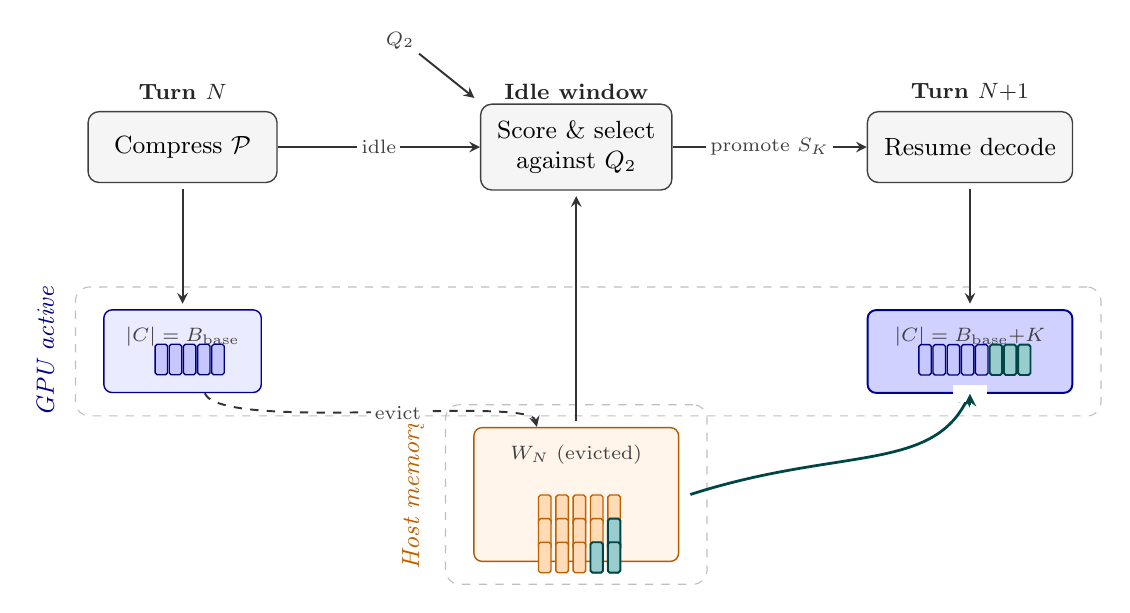
\begin{tikzpicture}[
  >=latex, line width=0.5pt,
  op/.style={rounded corners=4pt, draw=black!75, fill=gray!8,
             align=center, inner sep=6pt, font=\small,
             minimum width=2.4cm, minimum height=0.9cm},
  store/.style={rounded corners=3pt, draw=orange!70!black, fill=orange!8,
                inner sep=4pt, minimum height=1.7cm, align=center,
                font=\small},
  cache/.style={rounded corners=3pt, draw=blue!55!black, fill=blue!8,
                inner sep=4pt, minimum height=1.05cm, align=center,
                font=\small},
  cacheout/.style={cache, fill=blue!18, line width=0.7pt},
  chip/.style={rounded corners=0.7pt, minimum width=4.5pt, minimum height=11pt,
               inner sep=0pt, line width=0.5pt},
  gpuchip/.style={chip, draw=blue!50!black, fill=blue!22},
  hostchip/.style={chip, draw=orange!75!black, fill=orange!28},
  promchip/.style={chip, draw=teal!55!black, fill=teal!40, line width=0.7pt},
  rowband/.style={rounded corners=5pt, draw=gray!50, dashed, line width=0.4pt},
  bandlabel/.style={font=\itshape\small, text=black!70},
  arr/.style={->, line width=0.7pt, draw=black!80, >=stealth},
  promarr/.style={->, line width=1pt, draw=teal!55!black, >=stealth},
  arrlabel/.style={font=\scriptsize, fill=white, inner sep=1.5pt, text=black!75},
  collabel/.style={font=\bfseries\footnotesize, align=center, text=black!85},
  cellcap/.style={font=\scriptsize, text=black!75, align=center, anchor=north},
  anno/.style={font=\scriptsize, text=black!72, align=center}
]
  % --- Top: stage headers (single line above operator boxes, well-separated) ---
  \node[collabel] (h1) at (0, 4.7) {Turn $N$};
  \node[collabel] (h2) at (5.0, 4.7) {Idle window};
  \node[collabel] (h3) at (10.0, 4.7) {Turn $N{+}1$};

  % --- Operator pipeline: all three same fill (consistent operator class) ---
  \node[op] (compress) at (0, 4.0) {Compress~$\mathcal{P}$};
  \node[op] (score) at (5.0, 4.0)
       {Score \& select\\against $Q_2$};
  \node[op] (resume) at (10.0, 4.0) {Resume decode};

  \draw[arr] (compress) -- (score) node[arrlabel, midway] {idle};
  \draw[arr] (score) -- (resume) node[arrlabel, midway] {promote $S_K$};

  % --- Q_2 input: enters Score from UPPER-LEFT corner, label well clear of header ---
  \draw[arr] ([xshift=-22pt, yshift=18pt]score.north west)
             -- ([xshift=-2pt, yshift=2pt]score.north west);
  \node[arrlabel, anchor=south east]
       at ([xshift=-22pt, yshift=18pt]score.north west) {$Q_2$};

  % --- GPU active cache (Cbase) below compress ---
  \node[cache, minimum width=2.0cm, anchor=north] (cbase)
       at ([yshift=-1.6cm]compress.south) {};
  \node[cellcap] at ([yshift=-3pt]cbase.north)
       {$|C|=\bbase$};
  \foreach \i in {1,...,5}{
    \pgfmathsetmacro{\xc}{0.18*\i-0.45}
    \node[gpuchip] at ([xshift=\xc cm,yshift=-3pt]cbase.center) {};
  }

  % --- Host evicted store W_N: pushed BELOW the GPU row so tier bands don't overlap ---
  \node[store, minimum width=2.6cm, anchor=north] (wn)
       at ([yshift=-3.0cm]score.south) {};
  \node[cellcap] at ([yshift=-3pt]wn.north) {$W_N$ (evicted)};
  \foreach \i in {1,...,5}{
    \foreach \r in {0,1,2}{
      \pgfmathsetmacro{\xh}{0.22*\i-0.62}
      \pgfmathsetmacro{\yh}{-0.20-0.30*\r}
      \node[hostchip] at ([xshift=\xh cm,yshift=\yh cm]wn.center) {};
    }
  }
  % Three S_K candidates highlighted inside W_N (right side, illustrating selection)
  \pgfmathsetmacro{\xPa}{0.22*4-0.62} \pgfmathsetmacro{\yPa}{-0.20-0.30*2}
  \pgfmathsetmacro{\xPb}{0.22*5-0.62} \pgfmathsetmacro{\yPb}{-0.20-0.30*1}
  \pgfmathsetmacro{\xPc}{0.22*5-0.62} \pgfmathsetmacro{\yPc}{-0.20-0.30*2}
  \node[promchip] at ([xshift=\xPa cm,yshift=\yPa cm]wn.center) {};
  \node[promchip] at ([xshift=\xPb cm,yshift=\yPb cm]wn.center) {};
  \node[promchip] at ([xshift=\xPc cm,yshift=\yPc cm]wn.center) {};

  % --- Repaired GPU cache (post-promote) below resume ---
  \node[cacheout, minimum width=2.6cm, anchor=north] (crep)
       at ([yshift=-1.6cm]resume.south) {};
  \node[cellcap] at ([yshift=-3pt]crep.north)
       {$|C|=\bbase{+}K$};
  \foreach \i in {1,...,5}{
    \pgfmathsetmacro{\xc}{0.18*\i-0.75}
    \node[gpuchip] at ([xshift=\xc cm,yshift=-3pt]crep.center) {};
  }
  \foreach \i in {1,2,3}{
    \pgfmathsetmacro{\xs}{0.18*5+0.18*\i-0.75}
    \node[promchip] at ([xshift=\xs cm,yshift=-3pt]crep.center) {};
  }

  % --- Tier bands (dashed, behind cells); now non-overlapping in y ---
  \begin{scope}[on background layer]
    \node[rowband, fit=(cbase)(crep), inner xsep=10pt, inner ysep=8pt] (gband) {};
    \node[rowband, fit=(wn), inner xsep=10pt, inner ysep=8pt] (hband) {};
  \end{scope}
  % Tier labels: rotated 90 on the LEFT outside each band (truly consistent,
  % no overlap potential with cells or arrows).
  \node[bandlabel, anchor=south, text=blue!55!black, rotate=90]
       at ([xshift=-4pt]gband.west) {GPU active};
  \node[bandlabel, anchor=south, text=orange!75!black, rotate=90]
       at ([xshift=-4pt]hband.west) {Host memory};

  % --- Vertical state arrows ---
  % retain: just the arrow, label dropped (direction is self-evident)
  \draw[arr] ([yshift=-2pt]compress.south) -- ([yshift=2pt]cbase.north);
  % NEW: vertical connector under Resume decode (mirrors Compress -> Cbase)
  \draw[arr] ([yshift=-2pt]resume.south) -- ([yshift=2pt]crep.north);
  % evict: dashed, drops from cbase down to W_N top edge (not corner)
  \draw[arr,dashed] ([xshift=8pt]cbase.south)
       .. controls ([xshift=14pt,yshift=-0.5cm]cbase.south)
                  and ([xshift=-0.6cm,yshift=0.4cm]wn.north) ..
       ([xshift=-0.5cm]wn.north)
       node[arrlabel, pos=0.55] {evict};
  % score reads W_N: arrow from W_N top into score box
  \draw[arr] ([yshift=2pt]wn.north) -- ([yshift=-2pt]score.south);

  % --- Promote arrow (host -> repaired cache); anchors OUTSIDE W_N right edge.
  %     White halo punched where it crosses the GPU-active dashed band.
  \draw[promarr] ([xshift=4pt]wn.east)
       .. controls ([xshift=2.0cm,yshift=0.6cm]wn.east) and
                   ([xshift=-0.5cm,yshift=-1.0cm]crep.south) ..
       (crep.south);
  % Mask the gband bottom edge where the promote arrow enters crep so the
  % dashed line doesn't compete with the arrow visually.
  \fill[white] ([xshift=-6pt, yshift=-3pt]crep.south)
               rectangle ([xshift=6pt, yshift=3pt]crep.south);
  % redraw arrowhead on top of the mask
  \draw[promarr] ([yshift=-4pt]crep.south) -- (crep.south);
\end{tikzpicture}
\end{document}
